\documentclass[10pt,a4paper,UTF8]{ctexart}

\linespread{1.5}
\usepackage{geometry}%用于设置上下左右页边距
	\geometry{left=2.5cm,right=2.5cm,top=3.2cm,bottom=2.7cm}
\usepackage{xeCJK,amsmath,paralist,enumerate,booktabs,multirow,graphicx,subfig,setspace,listings,lastpage,hyperref}
\usepackage{amsthm, amssymb, bm, color, framed, graphicx, hyperref, mathrsfs}
\usepackage{mathrsfs}  
	\setlength{\parindent}{2em}
	\lstset{language=Matlab}%
\usepackage{fancyhdr}
\usepackage{graphicx}
\usepackage{subfloat}
\usepackage{listings}
\usepackage{xcolor}
\usepackage{float}
\usepackage{paralist}
\usepackage{setspace}
\usepackage{titlesec}
\usepackage{enumitem}
\usepackage{hyperref}
\usepackage{multirow}
\usepackage{threeparttable}
\usepackage{tcolorbox}
\usepackage{tabularx}
\usepackage{ulem}
\usepackage{multicol}
\usepackage{multirow}
\usepackage{pifont}


\hypersetup{
	colorlinks=true,
	linkcolor=black
}

\setenumerate{partopsep=0pt,topsep=0pt}
\setitemize{itemsep=0pt,partopsep=0pt,topsep=0pt}

\titlespacing*{\section}{0pt}{3pt}{3pt}
\titlespacing*{\subsection}{0pt}{2pt}{2pt}
\titlespacing*{\subsubsection}{0pt}{1pt}{1pt}
\titlespacing*{\paragraph}{0pt}{0pt}{0pt}

\ctexset{secnumdepth=4,tocdepth=4}
\setlength{\parindent}{2pt}
\setstretch{1.2}


\setCJKmainfont[BoldFont={FZHei-B01},ItalicFont={FZKai-Z03}]{FZShuSong-Z01} 
\setCJKsansfont[BoldFont={FZHei-B01}]{FZKai-Z03} 
\setCJKmonofont[BoldFont={FZHei-B01}]{FZFangSong-Z02}
\setCJKfamilyfont{zhsong}{FZShuSong-Z01} 
\setCJKfamilyfont{zhhei}{FZHei-B01} 
\setCJKfamilyfont{zhkai}[BoldFont={FZHei-B01}]{FZKai-Z03} 
\setCJKfamilyfont{zhfs}[BoldFont={FZHei-B01}]{FZFangSong-Z02} 
\renewcommand*{\songti}{\CJKfamily{zhsong}} 
\renewcommand*{\heiti}{\CJKfamily{zhhei}} 
\renewcommand*{\kaishu}{\CJKfamily{zhkai}} 
\renewcommand*{\fangsong}{\CJKfamily{zhfs}}

\newcommand{\myline}{\underline{\hbox to 10mm{}}}

\definecolor{mKeyword}{RGB}{0,0,255}          % bule
\definecolor{mString}{RGB}{160,32,240}        % purple
\definecolor{mComment}{RGB}{34,139,34}        % green
\definecolor{mNumber}{RGB}{128,128,128} 

\lstdefinestyle {njulisting} {
	basewidth = 0.5 em,
	lineskip = 3 pt,
	basicstyle = \small\ttfamily,
	% keywordstyle = \bfseries,
	commentstyle = \itshape\color{gray}, 
	basicstyle=\small\ttfamily,
	keywordstyle={\color{mKeyword}},     % sets color for keywords
	stringstyle={\color{mString}},       % sets color for strings
	commentstyle={\color{mComment}},     % sets color for comments
	numberstyle=\tiny\color{mNumber},
	numbers = left,
	captionpos = t,
	breaklines = true,
	xleftmargin = 2 em,
	xrightmargin = 2 em,
	frame=tlrb,
	tabsize=4
}

\lstset{
style = njulisting, % 调用上述样式 
flexiblecolumns % 允许调整字符宽度
}


%================= 基本格式预置 ===========================
\usepackage{fancyhdr}
\pagestyle{fancy}
\lhead{操作系统}
\rhead{MOOC习题答案}
\cfoot{\thepage}
\renewcommand{\headrulewidth}{0.4pt}
\renewcommand{\theenumi}{(\arabic{enumi})}
\CTEXsetup[format={\bfseries\zihao{-3}}]{section}
\CTEXsetup[format={\bfseries\zihao{4}}]{subsection}
\CTEXsetup[format={\bfseries\zihao{-4}}]{subsubsection}


\renewcommand{\contentsname}{目录}  

%\definecolor{shadecolor}{RGB}{241, 241, 255}
\newcounter{problemname}
\newenvironment{problem}{\stepcounter{problemname}\par\noindent\textbf{\arabic{problemname}. }}{\par}
\newenvironment{solution}{\noindent\textbf{解答:}}{\par}

\begin{document}

\setlength{\parskip}{0.65em}

\begin{center}
\LARGE\textbf{操作系统MOOC习题答案}
\end{center}

\subsection*{第一次习题}
\setcounter{problemname}{0}

\begin{problem}
	操作系统是对 \myline 进行管理的软件。
	\textbf{B}
	\vspace{-0.5em}
	\begin{multicols}{4}
		\begin{enumerate}[label=\Alph*.]
			\item 软件
			\item 计算机资源
			\item 硬件
			\item 应用程序
		\end{enumerate}
	\end{multicols}
	\vspace{-1em}
\end{problem}


\begin{problem}
	配置了操作系统的机器是一台比原来的物理机器功能更强的计算机,这样的计算机只是一台逻辑上的计算机,称为 \myline 计算机。
	\textbf{B}
	\vspace{-0.5em}
	\begin{multicols}{4}
		\begin{enumerate}[label=\Alph*.]
			\item 并行
			\item 虚拟
			\item 共享
			\item 真实
		\end{enumerate}
	\end{multicols}
	\vspace{-1em}
\end{problem}


\begin{problem}
	\myline 不是一个操作系统环境。
	\textbf{C}
	\vspace{-0.5em}
	\begin{multicols}{4}
		\begin{enumerate}[label=\Alph*.]
			\item Windows CE
			\item Solaris
			\item Celeron
			\item Linuxs
		\end{enumerate}
	\end{multicols}
	\vspace{-1em}
\end{problem}


\begin{problem}
	\myline 该操作系统的系统响应时间的重要性超过协同资源的利用率,它被广泛地应用于卫星控制、导弹发射、工业控制、飞机订票业务等领域。
	\textbf{C}
	\vspace{-0.5em}
	\begin{multicols}{4}
		\begin{enumerate}[label=\Alph*.]
			\item 多用户操作系统
			\item 分时操作系统
			\item 实时操作系统
			\item 批处理操作系统			
		\end{enumerate}
	\end{multicols}
	\vspace{-1em}
\end{problem}


\begin{problem}
	允许在一台主机上同时连接多个终端,各个用户可以通过各自的终端交互使用计算机,这样的操作系统是 \myline 。
	\textbf{D}
	\vspace{-0.5em}
	\begin{multicols}{4}
		\begin{enumerate}[label=\Alph*.]
			\item 网络操作系统
			\item 分布式操作系统
			\item 批处理操作系统
			\item 分时操作系统
		\end{enumerate}
	\end{multicols}
	\vspace{-1em}
\end{problem}


\begin{problem}
	如果分时系统的时间片一定,那么 \myline,则响应时间越长。
	\textbf{B}
	\vspace{-0.5em}
	\begin{multicols}{4}
		\begin{enumerate}[label=\Alph*.]
			\item 内存越多
			\item 用户数越多
			\item 内存越少
			\item 用户数越少
		\end{enumerate}
	\end{multicols}
	\vspace{-1em}
\end{problem}


\begin{problem}
	系统调用是 \myline。
	\textbf{B}
	\vspace{-0.5em}
	\begin{multicols}{2}
		\begin{enumerate}[label=\Alph*.]
			\item 用户编写的一个子程序
			\item 操作系统向用户程序提供的接口
			\item 高级语言中的库程序
			\item 操作系统中的一条命令
		\end{enumerate}
	\end{multicols}
	\vspace{-1em}
\end{problem}


\begin{problem}
	‍实时操作系统必须在 \myline 内处理来自外部的事件。
	\textbf{A}
	\vspace{-0.5em}
	\begin{multicols}{4}
		\begin{enumerate}[label=\Alph*.]
			\item 规定时间
			\item 周转时间
			\item 响应时间
			\item 调度时间
		\end{enumerate}
	\end{multicols}
	\vspace{-1em}
\end{problem}


\begin{problem}
	‍‍实时系统 \myline 。
	\textbf{D}
	%\vspace{-0.5em}
	%\begin{multicols}{1}
		\begin{enumerate}[label=\Alph*.]
			\item 强调系统资源的利用率
			\item 是依赖人为干预的监督和控制系统
			\item 实质上是批处理系统和分时系统的结合
			\item 必须既要及时响应、快速处理,又要有高可靠性和安全性
		\end{enumerate}
	%\end{multicols}
	%\vspace{-1em}
\end{problem}


\begin{problem}
	‍用户程序的输入和输出操作实际上由 \myline 完成。
	\textbf{A}
	\vspace{-0.5em}
	\begin{multicols}{4}
		\begin{enumerate}[label=\Alph*.]
			\item 操作系统
			\item 标准库程序
			\item 编译系统
			\item 程序设计语言
		\end{enumerate}
	\end{multicols}
	\vspace{-1em}
\end{problem}


\begin{problem}
	在操作系统中,并发性是指 \myline。
	\textbf{D}
	\vspace{-0.5em}
	\begin{multicols}{2}
		\begin{enumerate}[label=\Alph*.]
			\item 若干个时间在不同的时间间隔内发生
			\item 若干个时间在不同时刻发生
			\item 若干个事件在同一时刻发生
			\item 若干个事件在同一时间间隔内发生
		\end{enumerate}
	\end{multicols}
	\vspace{-1em}
\end{problem}


\begin{problem}
	若把操作系统看成计算机系统资源的管理者,下面的 \myline 不属于操作系统所管理的资源。
	\textbf{C}
	\vspace{-0.5em}
	\begin{multicols}{4}
		\begin{enumerate}[label=\Alph*.]
			\item 程序
			\item CPU
			\item 中断
			\item 主存
		\end{enumerate}
	\end{multicols}
	\vspace{-1em}
\end{problem}



\begin{problem}
	多道程序设计是指 \myline。   
	\textbf{C}
	\vspace{-0.5em}
	\begin{multicols}{2}
		\begin{enumerate}[label=\Alph*.]
			\item 在分布系统中同一时刻运行多个程序
			\item 在实时系统中并发运行多个程序
			\item 在一台处理机上并发运行多个程序
			\item 在一台处理机上同一时刻运行多个程序
		\end{enumerate}
	\end{multicols}
	\vspace{-1em}
\end{problem}



\begin{problem}
	提高处理器资源利用率的关键技术是 \myline。
	\textbf{A}
	\vspace{-0.5em}
	\begin{multicols}{4}
		\begin{enumerate}[label=\Alph*.]
			\item 多道程序设计技术
			\item 交换技术
			\item SPOOLing技术
			\item 虚拟技术
		\end{enumerate}
	\end{multicols}
	\vspace{-1em}
\end{problem}



\begin{problem}
	操作系统中采用多道程序设计提高CPU和外部设备的 \myline。
	\textbf{C}
	\vspace{-0.5em}
	\begin{multicols}{4}
		\begin{enumerate}[label=\Alph*.]
			\item 可靠性
			\item 稳定性
			\item 利用率
			\item 兼容性
		\end{enumerate}
	\end{multicols}
	\vspace{-1em}
\end{problem}


\begin{problem}
	引入多道程序设计技术的前提条件之一是系统具有 \myline。
	\textbf{C}
	\vspace{-0.5em}
	\begin{multicols}{4}
		\begin{enumerate}[label=\Alph*.]
			\item 多个CPU
			\item 多个终端
			\item 中断功能
			\item 分时功能
		\end{enumerate}
	\end{multicols}
	\vspace{-1em}
\end{problem}



\begin{problem}
	当计算机提供了管态和目态时,\myline 必须在管态下执行。
	\textbf{B}
	\vspace{-0.5em}
	\begin{multicols}{2}
		\begin{enumerate}[label=\Alph*.]
			\item 把运算结果送入内存的指令
			\item 输入/输出指令
			\item 算术运算指令
			\item 从内存取数的指令
		\end{enumerate}
	\end{multicols}
	\vspace{-1em}
\end{problem}



\begin{problem}
    当CPU执行操作系统代码时,称处理机处于 \myline。
	\textbf{B}
	\vspace{-0.5em}
	\begin{multicols}{4}
		\begin{enumerate}[label=\Alph*.]
			\item 目态
			\item 管态
			\item 自由态
			\item 就绪态
		\end{enumerate}
	\end{multicols}
	\vspace{-1em}
\end{problem}



\begin{problem}
	特权指令是指 \myline。
	\textbf{C}
	\vspace{-0.5em}
	\begin{multicols}{2}
		\begin{enumerate}[label=\Alph*.]
			\item 控制指令
			\item 系统管理员可用的指令;
			\item 其执行可能有损系统的安全性
			\item 机器指令
		\end{enumerate}
	\end{multicols}
	\vspace{-1em}
\end{problem}


\begin{problem}
	计算机系统中判断是否有中断事件发生应该在 \myline。
	\textbf{D}
	\vspace{-0.5em}
	\begin{multicols}{2}
		\begin{enumerate}[label=\Alph*.]
			\item 执行P操作后
			\item 由用户态转入核心态时
			\item 若干个事件在同一时刻发生
			\item 执行完一条指令后
		\end{enumerate}
	\end{multicols}
	\vspace{-1em}
\end{problem}
\subsection*{第二次习题}
\setcounter{problemname}{0}

\begin{problem}
	\myline 优先权是在创建进程时确定的,确定之后在整个进程运行期间不再改变。
	\textbf{B}
	\vspace{-0.5em}
	\begin{multicols}{4}
		\begin{enumerate}[label=\Alph*.]
			\item 动态
			\item 静态
			\item 短作业
			\item 先来先服务
		\end{enumerate}
	\end{multicols}
	\vspace{-1em}
\end{problem}


\begin{problem}
	下列进程状态变化中,\myline 变化是不可能发生的。
	\textbf{C}
	\vspace{-0.5em}
	\begin{multicols}{4}
		\begin{enumerate}[label=\Alph*.]
			\item 等待$\rightarrow$就绪
			\item 运行$\rightarrow$就绪
			\item 等待$\rightarrow$运行
			\item 运行$\rightarrow$等待
		\end{enumerate}
	\end{multicols}
	\vspace{-1em}
\end{problem}


\begin{problem}
	​当 \myline 时,进程从运行状态变为就绪状态。
	\textbf{D}
	\vspace{-0.5em}
	\begin{multicols}{2}
		\begin{enumerate}[label=\Alph*.]
			\item 进程被调度程序选中
			\item 等待某一事件
			\item 等待的事件发生
			\item 时间片到
		\end{enumerate}
	\end{multicols}
	\vspace{-1em}
\end{problem}


\begin{problem}
	进程管理中,当 \myline 时进程从阻塞态变成就绪态。
	\textbf{D}
	\vspace{-0.5em}
	\begin{multicols}{2}
		\begin{enumerate}[label=\Alph*.]
			\item 进程被进程调度程序选中
			\item 时间片用完
			\item 等待一个事件
			\item 等待的事件发生
		\end{enumerate}
	\end{multicols}
	\vspace{-1em}
\end{problem}


\begin{problem}
	下面对进程的描述中,错误的是 \myline。
	\textbf{A}
	\vspace{-0.5em}
	\begin{multicols}{2}
		\begin{enumerate}[label=\Alph*.]
			\item 进程是指令的集合
			\item 进程执行需要处理机
			\item 进程是有生命周期的
			\item 进程是动态的概念
		\end{enumerate}
	\end{multicols}
	\vspace{-1em}
\end{problem}


\begin{problem}
	下面所述步骤中,\myline 不是创建进程所必需的。
	\textbf{B}
	\vspace{-0.5em}
	\begin{multicols}{2}
		\begin{enumerate}[label=\Alph*.]
			\item 建立一个进程控制块
			\item 由调度程序为进程分配CPU
			\item 将进程控制块链入就绪队列
			\item 为进程分配内存
		\end{enumerate}
	\end{multicols}
	\vspace{-1em}
\end{problem}


\begin{problem}
	多道程序环境下,操作系统分配资源以 \myline 为基本单位。
	\textbf{A}
	\vspace{-0.5em}
	\begin{multicols}{4}
		\begin{enumerate}[label=\Alph*.]
			\item 进程
			\item 程序
			\item 线程
			\item 指令
		\end{enumerate}
	\end{multicols}
	\vspace{-1em}
\end{problem}


\begin{problem}
	下述哪一个选项体现了原语的主要特点 \myline。
	\textbf{A}
	\vspace{-0.5em}
	\begin{multicols}{4}
		\begin{enumerate}[label=\Alph*.]
			\item 不可分割性
			\item 共享性
			\item 并发性
			\item 异步性
		\end{enumerate}
	\end{multicols}
	\vspace{-1em}
\end{problem}


\begin{problem}
	‌关于内核级线程,以下描述不正确的是 \myline。
	\textbf{D}
		\begin{enumerate}[label=\Alph*.]
			\item 建立和维护线程的数据结构及保存每个线程的入口
			\item 内核可以将处理器调度直接分配给某个内核级线程
			\item 可以将一个进程的多个线程分派到多个处理器,能够发挥多处理器并行工作的优势
			\item 控制权从一个线程传送到另一个线程时不需要用户态—内核态—用户态的模式切换;
		\end{enumerate}
\end{problem}


\begin{problem}
	一个进程被唤醒意味着 \myline。
	\textbf{B}
	\vspace{-0.5em}
	\begin{multicols}{2}
		\begin{enumerate}[label=\Alph*.]
			\item 该进程重新占有了CPU
			\item 进程变为就绪状态
			\item 其PCB移至等待队列队首
			\item 它的优先权变为最大
		\end{enumerate}
	\end{multicols}
	\vspace{-1em}
\end{problem}


\begin{problem}
	在引入线程的操作系统中,资源分配的基本单位是 \myline。
	\textbf{D}
	\vspace{-0.5em}
	\begin{multicols}{4}
		\begin{enumerate}[label=\Alph*.]
			\item 作业
			\item 线程
			\item 程序
			\item 进程
		\end{enumerate}
	\end{multicols}
	\vspace{-1em}
\end{problem}


\begin{problem}
	在下述关于父进程和子进程的叙述中,正确的是 \myline。
	\textbf{B}
		\begin{enumerate}[label=\Alph*.]
			\item 父进程创建了子进程,因此父进程执行完了,子进程才能运行
			\item 父进程和子进程可以并发执行
			\item 撤销子进程时,应该同时撤销父进程
			\item 撤销父进程时,应该同时撤销子进程
		\end{enumerate}
\end{problem}


\begin{problem}
	对进程的管理和控制使用 \myline。
	\textbf{B}
	\vspace{-0.5em}
	\begin{multicols}{4}
		\begin{enumerate}[label=\Alph*.]
			\item 指令
			\item 原语
			\item 信号量
			\item 信箱通信
		\end{enumerate}
	\end{multicols}
	\vspace{-1em}
\end{problem}


\begin{problem}
	所谓“可重入”程序是指 \myline。
	\textbf{C}
	\vspace{-0.5em}
	\begin{multicols}{2}
		\begin{enumerate}[label=\Alph*.]
			\item 不能够被多个程序同时调用的程序
			\item 在执行过程中其代码自身会发生变化的程序
			\item 能够被多个进程共享的程序
			\item 无限循环程序
		\end{enumerate}
	\end{multicols}
	\vspace{-1em}
\end{problem}


\begin{problem}
	原语是 \myline。
	\textbf{C}
	\vspace{-0.5em}
	\begin{multicols}{2}
		\begin{enumerate}[label=\Alph*.]
			\item 可中断的指令序列
			\item 运行在用户态下的过程
			\item 不可中断的指令序列
			\item 操作系统的内核
		\end{enumerate}
	\end{multicols}
	\vspace{-1em}
\end{problem}


\begin{problem}
	在进程调度算法中,对短进程不利的是 \myline。
	\textbf{D}
	\vspace{-0.5em}
	\begin{multicols}{2}
		\begin{enumerate}[label=\Alph*.]
			\item 短进程优先调度算法
			\item 高响应比优先算法
			\item 多级反馈队列调度算法
			\item 先来先服务算法
		\end{enumerate}
	\end{multicols}
	\vspace{-1em}
\end{problem}


\begin{problem}
	一个可共享的程序在执行过程中是不能被修改的,这样的程序代码应该是 \myline。
	\textbf{B}
	\vspace{-0.5em}
	\begin{multicols}{4}
		\begin{enumerate}[label=\Alph*.]
			\item 封闭的代码
			\item 可重入代码
			\item 可执行代码
			\item 可再现代码
		\end{enumerate}
	\end{multicols}
	\vspace{-1em}
\end{problem}


\begin{problem}
	在进程管理中,当 \myline 时,进程状态从运行态转换到就绪态。
	\textbf{B}
	\vspace{-0.5em}
	\begin{multicols}{2}
		\begin{enumerate}[label=\Alph*.]
			\item 进程被调度程序选中
			\item 时间片用完
			\item 等待某一事件发生
			\item 等待的事件发生
		\end{enumerate}
	\end{multicols}
	\vspace{-1em}
\end{problem}


\begin{problem}
	Solaris的多线程的实现方式为 \myline。
	\textbf{A}
	\vspace{-0.5em}
	\begin{multicols}{4}
		\begin{enumerate}[label=\Alph*.]
			\item 混合式
			\item 纯用户级多线程
			\item 纯内核级线程
			\item 单线程结构进程
		\end{enumerate}
	\end{multicols}
	\vspace{-1em}
\end{problem}


\begin{problem}
	在UNIX系统中运行以下程序,最多可再产生出 \myline 进程?
	\textbf{D}
	\begin{lstlisting}
main( ){
   fork( ); /*←pc(程序计数器),进程A
   fork( );
   fork( );
}
	\end{lstlisting}
	\vspace{-0.5em}
	\begin{multicols}{4}
		\begin{enumerate}[label=\Alph*.]
			\item 3
			\item 9
			\item 5
			\item 7
		\end{enumerate}
	\end{multicols}
	\vspace{-1em}
\end{problem}
\subsection*{第三次习题}
\setcounter{problemname}{0}

\begin{problem}
	静态重定位的时机是 \myline。
	\textbf{B}
	\vspace{-0.5em}
	\begin{multicols}{4}
		\begin{enumerate}[label=\Alph*.]
			\item 程序编译时
			\item 程序装入时
			\item 程序链接时
			\item 程序运行时
		\end{enumerate}
	\end{multicols}
	\vspace{-1em}
\end{problem}


\begin{problem}
	‌能够装入内存任何位置的代码程序必须是\myline。
	\textbf{B}
	\vspace{-0.5em}
	\begin{multicols}{4}
		\begin{enumerate}[label=\Alph*.]
			\item 可定位的
			\item 可动态链接的
			\item 可重入的
			\item 可静态链接的
		\end{enumerate}
	\end{multicols}
	\vspace{-1em}
\end{problem}


\begin{problem}
	在可变式分区管理中,采用内存移动技术的目的是 \myline。
	\textbf{D}
	\vspace{-0.5em}
	\begin{multicols}{4}
		\begin{enumerate}[label=\Alph*.]
			\item 合并分配区
			\item 便于地址转换
			\item 增加主存容量
			\item 合并空闲区
		\end{enumerate}
	\end{multicols}
	\vspace{-1em}
\end{problem}


\begin{problem}
	在存储管理中,采用覆盖与交换技术的目的是 \myline。
	\textbf{B}
	\vspace{-0.5em}
	\begin{multicols}{2}
		\begin{enumerate}[label=\Alph*.]
			\item 物理上扩充主存容量
			\item 减少程序占用的主存空间
			\item 代码在主存中共享
			\item 提高CPU效率
		\end{enumerate}
	\end{multicols}
	\vspace{-1em}
\end{problem}


\begin{problem}
	‍在分区存储管理中,下面的 \myline 最有可能使得高地址空间变成为大的空闲区。
	\textbf{A}
	\vspace{-0.5em}
	\begin{multicols}{4}
		\begin{enumerate}[label=\Alph*.]
			\item 首次适应法
			\item 循环首次适应法
			\item 最佳适应法
			\item 最坏适应法
		\end{enumerate}
	\end{multicols}
	\vspace{-1em}
\end{problem}


\begin{problem}
	以下哪种 \myline 存储管理能提供虚存。
	\textbf{B}
	\vspace{-0.5em}
	\begin{multicols}{4}
		\begin{enumerate}[label=\Alph*.]
			\item 分区方式
			\item 页式
			\item 覆盖
			\item 可重定位分区管理
		\end{enumerate}
	\end{multicols}
	\vspace{-1em}
\end{problem}


\begin{problem}
	在分页式虚存中,分页由 \myline 实现。
	\textbf{B}
	\vspace{-0.5em}
	\begin{multicols}{4}
		\begin{enumerate}[label=\Alph*.]
			\item 程序员
			\item 操作系统
			\item 编译器
			\item 系统调用
		\end{enumerate}
	\end{multicols}
	\vspace{-1em}
\end{problem}


\begin{problem}
	在虚拟页式存储管理方案中,下面 \myline 完成将页面调入内存的工作。
	\textbf{C}
	\vspace{-0.5em}
	\begin{multicols}{4}
		\begin{enumerate}[label=\Alph*.]
			\item 页面淘汰过程
			\item 紧缩技术利用
			\item 缺页中断处理
			\item 工作集模型应用
		\end{enumerate}
	\end{multicols}
	\vspace{-1em}
\end{problem}


\begin{problem}
	采用 \myline 不会产生内部碎片。
	\textbf{A}
	\vspace{-0.5em}
	\begin{multicols}{2}
		\begin{enumerate}[label=\Alph*.]
			\item 分段式存储管理
			\item 固定分区式存储管理
			\item 分页式存储管理
			\item 段页式
		\end{enumerate}
	\end{multicols}
	\vspace{-1em}
\end{problem}



\begin{problem}
	​采用 \myline 存储管理不会产生外部碎片。
	\textbf{C}
	\vspace{-0.5em}
	\begin{multicols}{4}
		\begin{enumerate}[label=\Alph*.]
			\item 分段式
			\item 虚拟分段式
			\item 分页式
			\item 可变分区
		\end{enumerate}
	\end{multicols}
	\vspace{-1em}
\end{problem}


\begin{problem}
	一台机器有48位虚地址和32位物理地址,若页长为8KB,如果设计一个反置页表,则有 \myline 个页表项。
	\textbf{B}
	\vspace{-0.5em}
	\begin{multicols}{4}
		\begin{enumerate}[label=\Alph*.]
			\item $2^{35}$
			\item $2^{19}$
			\item $2^{16}$
			\item $2^{32}$
		\end{enumerate}
	\end{multicols}
	\vspace{-1em}
\end{problem}


\begin{problem}
	作业在执行中发生了缺页中断,经操作系统处理后,应该让其执行 \myline 指令。
	\textbf{C}
	\vspace{-0.5em}
	\begin{multicols}{4}
		\begin{enumerate}[label=\Alph*.]
			\item 被中断的前一条
			\item 被中断的后一条
			\item 被中断的
			\item 启动时的第一条
		\end{enumerate}
	\end{multicols}
	\vspace{-1em}
\end{problem}


\begin{problem}
	在请求分页存储管理中,当访问的页面不在内存时,便产生缺页中断,缺页中断是属于 \myline。
	\textbf{B}
	\vspace{-0.5em}
	\begin{multicols}{4}
		\begin{enumerate}[label=\Alph*.]
			\item 外中断
			\item I/O中断
			\item 程序中断
			\item 访管中断
		\end{enumerate}
	\end{multicols}
	\vspace{-1em}
\end{problem}


\begin{problem}
	通常所说的"存储保护"的基本含义是 \myline。
	\textbf{D}
	\vspace{-0.5em}
	\begin{multicols}{2}
		\begin{enumerate}[label=\Alph*.]
			\item 防止存储器硬件受损
			\item 防止程序被人偷看
			\item 防止程序在内存丢失
			\item 防止程序间相互越界访问
		\end{enumerate}
	\end{multicols}
	\vspace{-1em}
\end{problem}


\begin{problem}
	LRU置换算法所基于的思想是 \myline。
	\textbf{A}
		\begin{enumerate}[label=\Alph*.]
			\item 在最近的过去很久未使用的在最近的将来也不会使用
			\item 在最近的过去用得多的在最近的将来也用得多
			\item 在最近的过去很久未使用的在最近的将来会使用
			\item 在最近的过去用得少的在最近的将来也用得少
		\end{enumerate}
\end{problem}


\begin{problem}
	在下面关于虚拟存储器的叙述中,正确的是 \myline。
	\textbf{D}
		\begin{enumerate}[label=\Alph*.]
			\item 要求程序运行前必须全部装入内存但在运行过程中不必一直驻留在内存
			\item 要求程序运行前不必全部装入内存但是在运行过程中必须一直驻留在内存
			\item 要求程序运行前必须全部装入内存且在运行过程中一直驻留在内存
			\item 要求程序运行前不必全部装入内存且在运行过程中不必一直驻留在内存
		\end{enumerate}
\end{problem}



\begin{problem}
	​虚存的可行性基础是 \myline。
	\textbf{D}
	\vspace{-0.5em}
	\begin{multicols}{4}
		\begin{enumerate}[label=\Alph*.]
			\item 程序执行的离散性
			\item 程序执行的并发性
			\item 程序执行的顺序性
			\item 程序执行的局部性
		\end{enumerate}
	\end{multicols}
	\vspace{-1em}
\end{problem}


\begin{problem}
	把逻辑地址转变为内存的物理地址的过程称作 \myline。
	\textbf{A}
	\vspace{-0.5em}
	\begin{multicols}{4}
		\begin{enumerate}[label=\Alph*.]
			\item 重定位或地址映射
			\item 运行
			\item 编译
			\item 连接
		\end{enumerate}
	\end{multicols}
	\vspace{-1em}
\end{problem}


\begin{problem}
	假定某页式管理系统中,主存128KB,分成32块,块号为$0,1,2,\dots,331$;某作业有5块,其页号为$0,1,2,3,4$,被分别装入主存的$3,8,4,6,9$块中。有一逻辑地址为$[3,70]$。试求出相应的物理地址 \myline (其中方括号中的第一个元素为页号,第二个元素为页内地址,按十进制计算)。
	\textbf{C}
	\vspace{-0.5em}
	\begin{multicols}{4}
		\begin{enumerate}[label=\Alph*.]
			\item 14646
			\item 34576
			\item 24646
			\item 24576
		\end{enumerate}
	\end{multicols}
	\vspace{-1em}
\end{problem}


\begin{problem}
	页面替换算法 \myline 有可能会产生Belady异常现象。
	\textbf{B}
	\vspace{-0.5em}
	\begin{multicols}{4}
		\begin{enumerate}[label=\Alph*.]
			\item Clock
			\item FIFO
			\item OPT
			\item LRU
		\end{enumerate}
	\end{multicols}
	\vspace{-1em}
\end{problem}
\subsection*{第四次习题}
\setcounter{problemname}{0}

\begin{problem}
	按 \myline 分类可将设备分为块设备和字符设备。
	\textbf{D}
	\vspace{-0.5em}
	\begin{multicols}{4}
		\begin{enumerate}[label=\Alph*.]
			\item 共享属性
			\item 操作特性
			\item 从属关系
			\item 信息交换单位
		\end{enumerate}
	\end{multicols}
	\vspace{-1em}
\end{problem}


\begin{problem}
	CPU输出数据的速度远远高于打印机的打印速度,为了解决这一矛盾,可采用 \myline。
	\textbf{A}
	\vspace{-0.5em}
	\begin{multicols}{4}
		\begin{enumerate}[label=\Alph*.]
			\item 缓冲技术
			\item 覆盖技术
			\item 虚存技术
			\item 并行技术
		\end{enumerate}
	\end{multicols}
	\vspace{-1em}
\end{problem}


\begin{problem}
	通过硬件和软件的功能扩充,把原来独占的设备改造成能为若干用户共享的设备,这种设备称为 \myline。
	\textbf{D}
	\vspace{-0.5em}
	\begin{multicols}{4}
		\begin{enumerate}[label=\Alph*.]
			\item 系统设备
			\item 存储设备
			\item 用户设备
			\item 虚拟设备
		\end{enumerate}
	\end{multicols}
	\vspace{-1em}
\end{problem}


\begin{problem}
	通道又称I/O处理机,它用于实现 \myline 之间的信息传输。
	\textbf{A}
	\vspace{-0.5em}
	\begin{multicols}{4}
		\begin{enumerate}[label=\Alph*.]
			\item 内存与外设
			\item 内存与外存
			\item CPU与外设
			\item CPU与外存
		\end{enumerate}
	\end{multicols}
	\vspace{-1em}
\end{problem}


\begin{problem}
	为了使多个进程能有效地同时处理输入和输出,最好使用 \myline 结构的缓冲技术。
	\textbf{B}
	\vspace{-0.5em}
	\begin{multicols}{4}
		\begin{enumerate}[label=\Alph*.]
			\item 单缓冲
			\item 缓冲池
			\item 双缓冲
			\item 循环缓冲
		\end{enumerate}
	\end{multicols}
	\vspace{-1em}
\end{problem}


\begin{problem}
	如果I/O设备与存储设备进行数据交换不经过CPU来完成,这种数据交换方式是 \myline。
	\textbf{A}
	\vspace{-0.5em}
	\begin{multicols}{4}
		\begin{enumerate}[label=\Alph*.]
			\item DMA方式
			\item 中断方式
			\item 无条件存取方式
			\item 程序轮询
		\end{enumerate}
	\end{multicols}
	\vspace{-1em}
\end{problem}


\begin{problem}
	​在中断处理中,输入/输出中断可能是指 \myline:\ding{192}设备出错,\ding{193}数据传输结束。
	\textbf{D}
	\vspace{-0.5em}
	\begin{multicols}{4}
		\begin{enumerate}[label=\Alph*.]
			\item \ding{193}
			\item \ding{192}
			\item 都不是
			\item \ding{192}和\ding{193}
		\end{enumerate}
	\end{multicols}
	\vspace{-1em}
\end{problem}


\begin{problem}
	在采用SPOOLing技术的系统中,用户的打印结果首先被送到 \myline。
	\textbf{D}
	\vspace{-0.5em}
	\begin{multicols}{4}
		\begin{enumerate}[label=\Alph*.]
			\item 打印机
			\item 终端
			\item 内存固定区域
			\item 磁盘固定区域
		\end{enumerate}
	\end{multicols}
	\vspace{-1em}
\end{problem}


\begin{problem}
	大多数低速设备都属于 \myline 设备。
	\textbf{C}
	\vspace{-0.5em}
	\begin{multicols}{4}
		\begin{enumerate}[label=\Alph*.]
			\item 虚拟
			\item SPOOLing
			\item 独享
			\item 共享
		\end{enumerate}
	\end{multicols}
	\vspace{-1em}
\end{problem}


\begin{problem}
	\myline 是直接存取的存储设备。
	\textbf{B}
	\vspace{-0.5em}
	\begin{multicols}{4}
		\begin{enumerate}[label=\Alph*.]
			\item 键盘显示终端
			\item 磁盘
			\item 磁带
			\item 打印机
		\end{enumerate}
	\end{multicols}
	\vspace{-1em}
\end{problem}


\begin{problem}
	操作系统中的SPOOLing技术,实质是指 \myline 转化为共享设备的技术。
	\textbf{A}
	\vspace{-0.5em}
	\begin{multicols}{4}
		\begin{enumerate}[label=\Alph*.]
			\item 独占设备
			\item 脱机设备
			\item 块设备
			\item 虚拟设备
		\end{enumerate}
	\end{multicols}
	\vspace{-1em}
\end{problem}


\begin{problem}
	在操作系统中,\myline 指的是一种硬件机制。
	\textbf{C}
	\vspace{-0.5em}
	\begin{multicols}{4}
		\begin{enumerate}[label=\Alph*.]
			\item SPOOLing技术
			\item 缓冲池
			\item 通道技术
			\item 内存覆盖技术
		\end{enumerate}
	\end{multicols}
	\vspace{-1em}
\end{problem}


\begin{problem}
	在操作系统中,用户程序申请使用I/O设备时,通常采用 \myline。
	\textbf{C}
	\vspace{-0.5em}
	\begin{multicols}{4}
		\begin{enumerate}[label=\Alph*.]
			\item 独占设备名
			\item 虚拟设备名
			\item 逻辑设备名
			\item 物理设备名
		\end{enumerate}
	\end{multicols}
	\vspace{-1em}
\end{problem}


\begin{problem}
	采用假脱机技术,将磁盘的一部分作为公共缓冲区以代替打印机,用户对打印机的操作实际上是对磁盘的存储操作,用以代替打印机的部分是 \myline。
	\textbf{B}
	\vspace{-0.5em}
	\begin{multicols}{4}
		\begin{enumerate}[label=\Alph*.]
			\item 独占设备
			\item 虚拟设备
			\item 一般物理设备
			\item 共享设备
		\end{enumerate}
	\end{multicols}
	\vspace{-1em}
\end{problem}


\begin{problem}
	\myline 算法是设备分配常用的一种算法。
	\textbf{C}
	\vspace{-0.5em}
	\begin{multicols}{4}
		\begin{enumerate}[label=\Alph*.]
			\item 首次适应
			\item 最佳适应
			\item 先来先服务
			\item 短作业优先
		\end{enumerate}
	\end{multicols}
	\vspace{-1em}
\end{problem}


\begin{problem}
	‌将系统中的每一台设备按某种原则进行统一的编号,这些编号作为区分硬件和识别设备的代号,该编号称为设备的 \myline。
	\textbf{D}
	\vspace{-0.5em}
	\begin{multicols}{4}
		\begin{enumerate}[label=\Alph*.]
			\item 符号名
			\item 相对号
			\item 类型号
			\item 绝对号
		\end{enumerate}
	\end{multicols}
	\vspace{-1em}
\end{problem}


\begin{problem}
	通道程序是 \myline。
	\textbf{C}
	\vspace{-0.5em}
	\begin{multicols}{2}
		\begin{enumerate}[label=\Alph*.]
			\item 可以由高级语言编写
			\item 由一系列机器指令组成
			\item 由一系列通道指令组成
			\item 就是通道控制器
		\end{enumerate}
	\end{multicols}
	\vspace{-1em}
\end{problem}


\begin{problem}
	I/O软件的分层结构中,\myline 负责将把用户提交的逻辑I/O请求转化为物理I/O操作的启动和执行。
	\textbf{B}
	\vspace{-0.5em}
	\begin{multicols}{2}
		\begin{enumerate}[label=\Alph*.]
			\item 独立于设备的I/O软件
			\item 设备驱动程序
			\item 用户空间的I/O软件
			\item I/O中断处理程序
		\end{enumerate}
	\end{multicols}
	\vspace{-1em}
\end{problem}


\begin{problem}
	使用SPOOLing系统的目的是为了提高 \myline 的使用效率。
	\textbf{B}
	\vspace{-0.5em}
	\begin{multicols}{4}
		\begin{enumerate}[label=\Alph*.]
			\item 操作系统
			\item I/O设备
			\item 内存
			\item CPU
		\end{enumerate}
	\end{multicols}
	\vspace{-1em}
\end{problem}


\begin{problem}
	下列算法中,用于磁盘移臂调度的是 \myline。
	\textbf{D}
	\vspace{-0.5em}
	\begin{multicols}{2}
		\begin{enumerate}[label=\Alph*.]
			\item 时间片轮转法
			\item 优先级高者优先算法
			\item LRU算法
			\item 最短寻找时间优先算法
		\end{enumerate}
	\end{multicols}
	\vspace{-1em}
\end{problem}

\subsection*{第五次习题}
\setcounter{problemname}{0}

\begin{problem}
	Unix系统中,文件的索引结构存放在 \myline 中。
	\textbf{D}
	\vspace{-0.5em}
	\begin{multicols}{4}
		\begin{enumerate}[label=\Alph*.]
			\item 超级块
			\item 空闲块
			\item 目录项
			\item inode节点
		\end{enumerate}
	\end{multicols}
	\vspace{-1em}
\end{problem}


\begin{problem}
	操作系统中对文件进行管理的部分叫做 \myline。
	\textbf{B}
	\vspace{-0.5em}
	\begin{multicols}{4}
		\begin{enumerate}[label=\Alph*.]
			\item 数据库系统
			\item 文件系统
			\item 检索系统
			\item 数据存储系统
		\end{enumerate}
	\end{multicols}
	\vspace{-1em}
\end{problem}


\begin{problem}
	为了解决不同用户文件的“命名冲突”问题,通常在文件系统中采用 \myline。
	\textbf{C}
	\vspace{-0.5em}
	\begin{multicols}{4}
		\begin{enumerate}[label=\Alph*.]
			\item 约定的方法
			\item 索引
			\item 多级目录
			\item 路径
		\end{enumerate}
	\end{multicols}
	\vspace{-1em}
\end{problem}


\begin{problem}
	无结构文件的含义是 \myline。
	\textbf{B}
	\vspace{-0.5em}
	\begin{multicols}{4}
		\begin{enumerate}[label=\Alph*.]
			\item 索引文件
			\item 流式文件
			\item 变长记录的文件
			\item 索引顺序文件
		\end{enumerate}
	\end{multicols}
	\vspace{-1em}
\end{problem}


\begin{problem}
	下列文件中不属于物理文件的是 \myline。
	\textbf{A}
	\vspace{-0.5em}
	\begin{multicols}{4}
		\begin{enumerate}[label=\Alph*.]
			\item 记录式文件
			\item 连续文件
			\item 链接文件
			\item 索引文件
		\end{enumerate}
	\end{multicols}
	\vspace{-1em}
\end{problem}


\begin{problem}
	文件系统的主要目的是 \myline。
	\textbf{B}
	\vspace{-0.5em}
	\begin{multicols}{2}
		\begin{enumerate}[label=\Alph*.]
			\item 实现虚拟存储
			\item 实现对文件的按名存取
			\item 用于存储系统文件
			\item 提高外存的读写速度
		\end{enumerate}
	\end{multicols}
	\vspace{-1em}
\end{problem}


\begin{problem}
	下列文件中属于逻辑结构的文件是 \myline 文件。
	\textbf{A}
	\vspace{-0.5em}
	\begin{multicols}{4}
		\begin{enumerate}[label=\Alph*.]
			\item 流式文件
			\item 库文件
			\item 连续文件
			\item 系统文件
		\end{enumerate}
	\end{multicols}
	\vspace{-1em}
\end{problem}


\begin{problem}
	文件系统采用多级目录结构后,对于不同用户的文件,其文件名 \myline。
	\textbf{A}
	\vspace{-0.5em}
	\begin{multicols}{2}
		\begin{enumerate}[label=\Alph*.]
			\item 可以相同也可以不同
			\item 受系统约束
			\item 应该不同
			\item 应该相同
		\end{enumerate}
	\end{multicols}
	\vspace{-1em}
\end{problem}


\begin{problem}
	文件目录的主要作用是 \myline。
	\textbf{C}
	\vspace{-0.5em}
	\begin{multicols}{4}
		\begin{enumerate}[label=\Alph*.]
			\item 节省空间
			\item 提高外存利用率
			\item 按名存取
			\item 提高速度
		\end{enumerate}
	\end{multicols}
	\vspace{-1em}
\end{problem}


\begin{problem}
	在文件系统中,文件的不同物理结构有不同的优缺点。在下列文件的物理结构中,\myline 具有直接读写文件任意一个记录的能力,又提高了文件存储空间的利用率。
	\textbf{A}
	\vspace{-0.5em}
	\begin{multicols}{4}
		\begin{enumerate}[label=\Alph*.]
			\item 索引结构
			\item Hash结构
			\item 顺序结构
			\item 链接结构
		\end{enumerate}
	\end{multicols}
	\vspace{-1em}
\end{problem}


\begin{problem}
	文件系统用 \myline 组织文件。
	\textbf{B}
	\vspace{-0.5em}
	\begin{multicols}{4}
		\begin{enumerate}[label=\Alph*.]
			\item 堆栈
			\item 目录
			\item 路径
			\item 指针
		\end{enumerate}
	\end{multicols}
	\vspace{-1em}
\end{problem}


\begin{problem}
	文件路径名是指 \myline。
	\textbf{B}
		\begin{enumerate}[label=\Alph*.]
			\item 目录文件名和文件名的集合
			\item 从根目录到文件所经历的路径中的各符号名的集合
			\item 文件名和文件扩展名
			\item 一系列的目录文件名和该文件的文件名
		\end{enumerate}
\end{problem}


\begin{problem}
	一个文件的相对路径名是从 \myline 开始,逐步沿着各级子目录追溯,最后到指定文件的整个通路上所有子目录名组成的一个字符串。
	\textbf{A}
	\vspace{-0.5em}
	\begin{multicols}{4}
		\begin{enumerate}[label=\Alph*.]
			\item 当前目录
			\item 二级目录
			\item 根目录
			\item 多级目录
		\end{enumerate}
	\end{multicols}
	\vspace{-1em}
\end{problem}


\begin{problem}
	对一个文件的访问,常由 \myline 共同限制。
	\textbf{C}
	\vspace{-0.5em}
	\begin{multicols}{2}
		\begin{enumerate}[label=\Alph*.]
			\item 文件属性的口令
			\item 优先级和文件属性
			\item 用户访问权限和文件属性
			\item 用户访问权限和用户优先级
		\end{enumerate}
	\end{multicols}
	\vspace{-1em}
\end{problem}


\begin{problem}
	存放在磁盘上的文件 \myline。
	\textbf{C}
	\vspace{-0.5em}
	\begin{multicols}{2}
		\begin{enumerate}[label=\Alph*.]
			\item 不能随机访问
			\item 只能顺序访问
			\item 既可随机访问,又可顺序访问
			\item 只能随机访问
		\end{enumerate}
	\end{multicols}
	\vspace{-1em}
\end{problem}


\begin{problem}
	在文件系统中,位示图可用于 \myline。
	\textbf{C}
	\vspace{-0.5em}
	\begin{multicols}{2}
		\begin{enumerate}[label=\Alph*.]
			\item 内存空间的共享
			\item 实现文件的保护和保密
			\item 磁盘空间的管理
			\item 文件目录的查找
		\end{enumerate}
	\end{multicols}
	\vspace{-1em}
\end{problem}


\begin{problem}
	常用的文件存取方法有两种:顺序存取和 \myline 存取。
	\textbf{B}
	\vspace{-0.5em}
	\begin{multicols}{4}
		\begin{enumerate}[label=\Alph*.]
			\item 顺序
			\item 随机
			\item 串联
			\item 流式
		\end{enumerate}
	\end{multicols}
	\vspace{-1em}
\end{problem}


\begin{problem}
	Unix系统中,通过 \myline 实现文件系统的按名存取功能。
	\textbf{A}
	\vspace{-0.5em}
	\begin{multicols}{4}
		\begin{enumerate}[label=\Alph*.]
			\item 目录项
			\item 超级块
			\item 空闲块
			\item inode节点
		\end{enumerate}
	\end{multicols}
	\vspace{-1em}
\end{problem}


\begin{problem}
	Unix文件系统中,打开文件的系统调用open输入参数包含 \myline。
	\textbf{A}
	\vspace{-0.5em}
	\begin{multicols}{4}
		\begin{enumerate}[label=\Alph*.]
			\item 文件名
			\item 文件描述符
			\item inode
			\item inode号
		\end{enumerate}
	\end{multicols}
	\vspace{-1em}
\end{problem}


\begin{problem}
	Unix文件系统中,打开文件的系统调用open返回值是 \myline。
	\textbf{A}
	\vspace{-0.5em}
	\begin{multicols}{4}
		\begin{enumerate}[label=\Alph*.]
			\item 文件描述符(字)
			\item inode
			\item 文件名
			\item inode号
		\end{enumerate}
	\end{multicols}
	\vspace{-1em}
\end{problem}

\subsection*{期末测试}
\setcounter{problemname}{0}

\begin{problem}
试写出进程映像包括哪些组成部分。
\end{problem}

\begin{solution}
进程控制块、进程程序块、进程数据块和进程核心栈。
\end{solution}


\begin{problem}
I/O软件的一般分为四层结构,请按照自顶向下的顺序写出四层结构的名称。
\end{problem}
    
\begin{solution}
    用户空间的I/O软件;独立于设备的I/O软件;设备驱动程序;中断处理程序。
\end{solution}


\begin{problem}
假设一个可移动磁头的磁盘具有200个磁道,编号为0$\sim$199,刚结束了175道的存取,正在处理143道的服务请求,假设系统当前I/O请求队列如下:85,145,90,180,92,150,102,176,132。试问:如果采用电梯调度算法完成上述请求,其存取臂移动的总量是多少?并写出磁头臂移动的序列。
\end{problem}

\begin{solution}
    磁头移动序列为132$\rightarrow$\,102$\rightarrow$\,92$\rightarrow$\,90$\rightarrow$\,85$\rightarrow$\,145$\rightarrow$\,150$\rightarrow$\,176$\rightarrow$\,180

    存取臂移动的总量为$(143-85)+(180-85)=153$
\end{solution}


\begin{problem}
请画出或描述出七状态进程模型(含两个挂起状态)及其状态转换图。
\end{problem}

\begin{solution}
    \begin{figure}[H]
        \vspace{-0.5em}
        \centering
        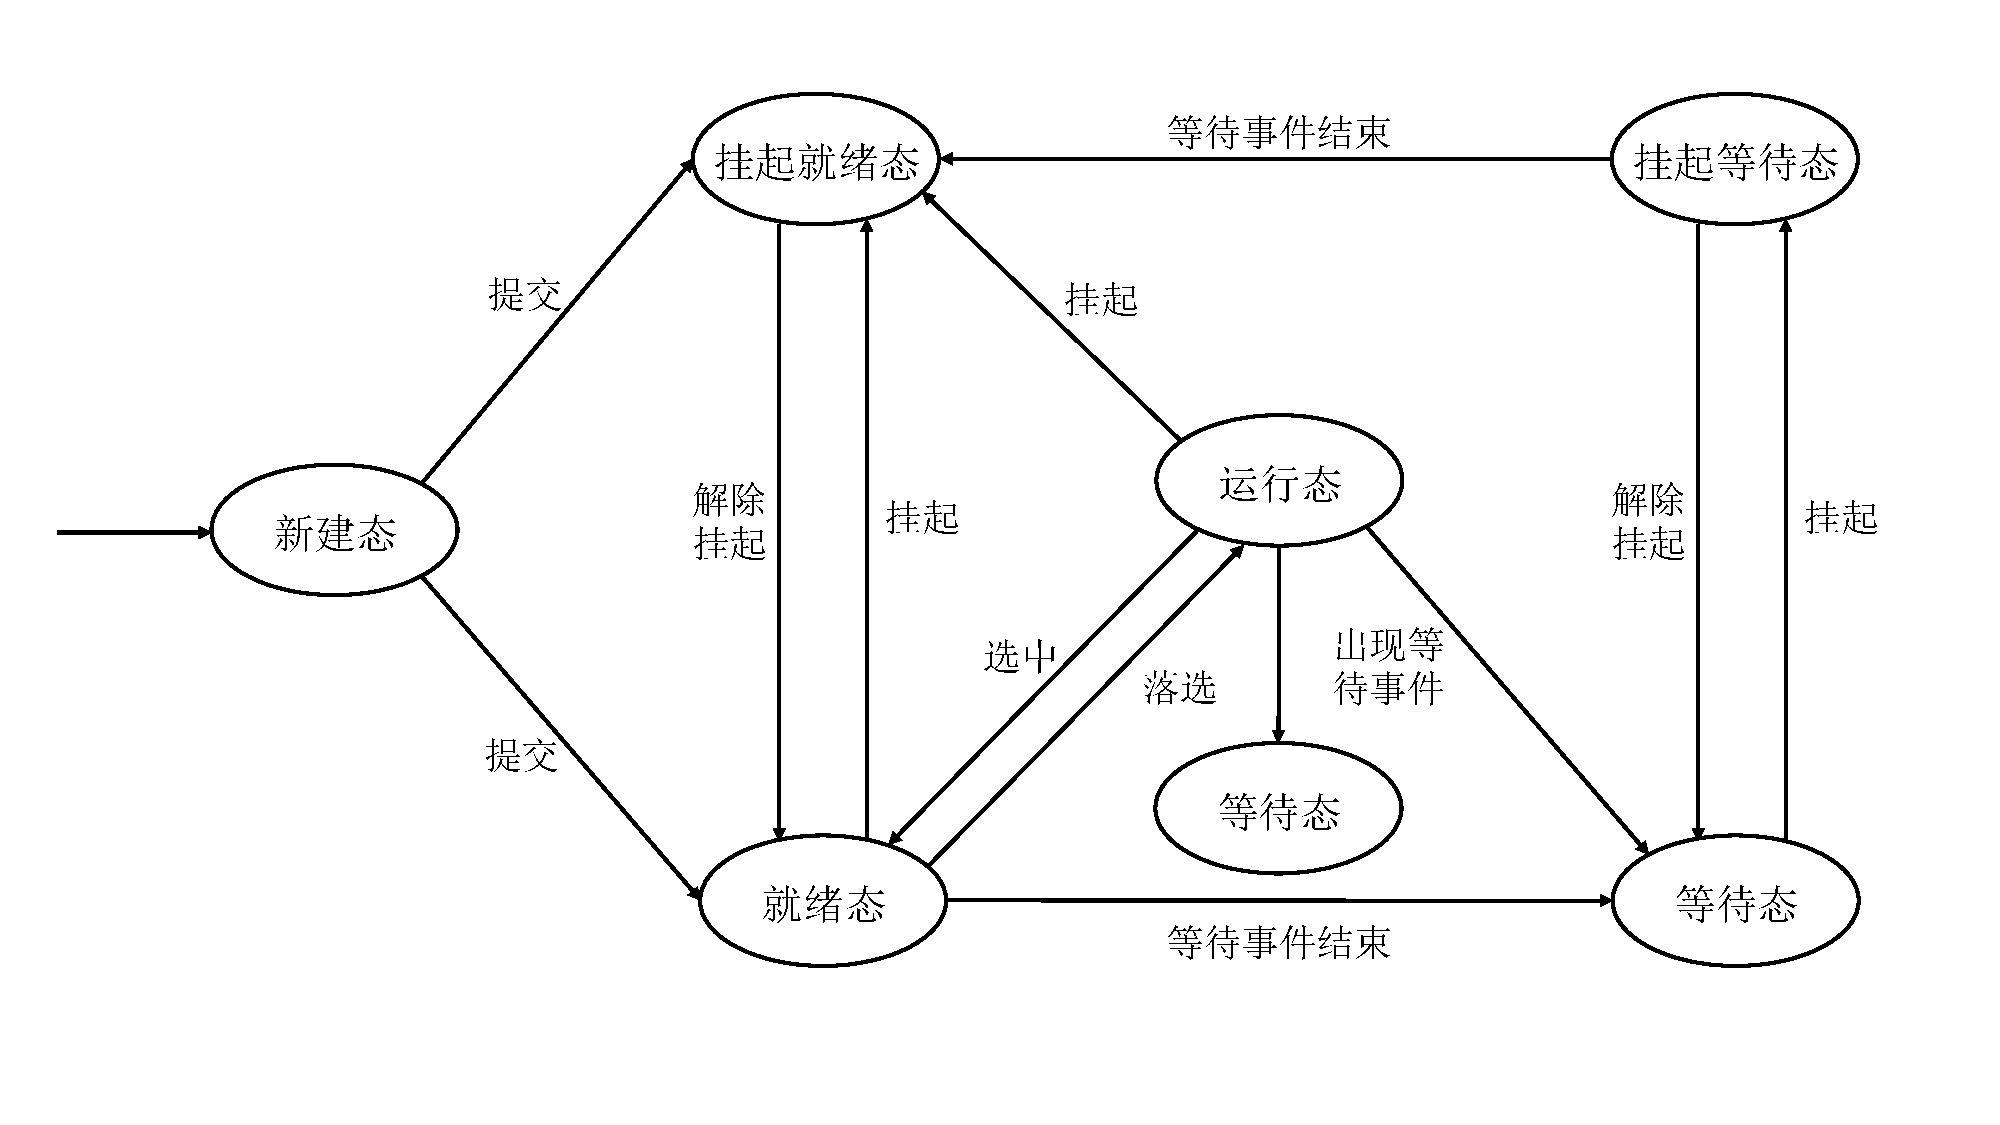
\includegraphics[width=0.7\linewidth]{七状态进程模型.pdf}
        \vspace{-1em}
    \end{figure}
\end{solution}



\begin{problem}
一台机器有48位虚地址和32位物理地址,若页长为4KB,问如果采用正向页表,一个进程的页表最多有多少个页表项? 如果设计一个反置页表,则有多少个页表项?
\end{problem}

\begin{solution}
    由于页长为4KB($2^{12}$B),所以页内偏移量为12位,所以页表项共有$2^{48-12}=2^{36}$个,反置页表项共有$2^{32-12}=2^{20}$个。
\end{solution}


\begin{problem}
 在UNIX系统中,每个$i$节点中分别含有12个直接地址的索引和一、二、三级间接索引。假设每个盘块有1024Byte,若每个盘块放256个盘块地址,50MB的文件和100MB的文件分别占用多少直接、一、二、三级间接盘块?
\end{problem}

\begin{solution}
直接盘块容量:$1024\mathrm{B}\times 12=12\mathrm{KB}$

一级间接盘块容量:$256 \times 1024\mathrm{B}=256\mathrm{KB}$

二级间接盘块容量:$256 \times 256\mathrm{KB}=65536\mathrm{KB}=64\mathrm{MB}$

三级间接盘块容量:$64\mathrm{MB} \times 256=16384\mathrm{MB}$

50MB的文件占用12个直接盘块和256个一级间接盘块,二级间接盘块占用数量为$(50\mathrm{MB}-12\mathrm{KB}-256\mathrm{KB})\div 1024\mathrm{B}=50932$个

100MB的文件占用12个直接盘块、256个一级间接盘块和$256\times 256=65536$个二级间接盘块,三级间接盘块的占用数量为$(100\mathrm{MB}-12\mathrm{KB}-256\mathrm{KB}-64\mathrm{MB})\div 1024\mathrm{B}=36596$个

\end{solution}


\begin{problem}
考虑下面的进程集合:
\begin{table}[H]
    \vspace{-0.5em}
    \centering
    \begin{tabular}{|c|c|c|}
    \hline
    进程& 到达时间& 处理时间\\ \hline
    A & 0   & 2   \\ \hline
    B & 1   & 8   \\ \hline
    C & 2   & 2   \\ \hline
    D & 3   & 8   \\ \hline
    \end{tabular}
    \vspace{-1.5em}
\end{table}
如果使用先来先服务FCFS调度算法,得到的每个单位时间内的进程执行序列表示为:
\begin{table}[H]
    \vspace{-0.5em}
    \centering
    \resizebox{\linewidth}{!}{
    \begin{tabular}{|c|c|c|c|c|c|c|c|c|c|c|c|c|c|c|c|c|c|c|c|c|}
    \hline
    算法  & 1   & 2   & 3   & 4   & 5   & 6   & 7   & 8   & 9   & 10  & 11  & 12  & 13  & 14  & 15  & 16  & 17  & 18  & 19  & 20  \\ \hline
    FCFS & A & A & B & B & B & B & B & B & B & B & C & C & D & D & D & D & D & D & D & D \\ \hline
    \end{tabular}
    }
    \vspace{-1.5em}
\end{table}
参照该FCFS调度算法给出的执行序列的写法,写出如果采用时间片轮转RR(时间片单位$q=1, q=4$)、多级反馈队列Feedback(反馈Fback,$q=1$;Fback,$q=2^i$)等4个调度算法,得到进程执行序列。注:在时间片轮转或者多级反馈队列调度时,如果就绪队列都为空,正在运行的进程不被抢占,继续使用下一段时间片。

\end{problem}

\begin{solution}
    \begin{table}[H]
        \vspace{-0.5em}
        \centering
        \resizebox{\linewidth}{!}{
        \begin{tabular}{|c|c|c|c|c|c|c|c|c|c|c|c|c|c|c|c|c|c|c|c|c|}
        \hline
        算法          & 1    & 2    & 3    & 4    & 5    & 6    & 7    & 8    & 9    & 10   & 11   & 12   & 13   & 14   & 15   & 16   & 17   & 18   & 19   & 20   \\ \hline
        RR,$q=1$     &  A  & B  &  A &  C &  B &  D &  C &  B &  D & B  &  D &  B &  D &  B &  D &  B & D  &  B &  D &  D \\ \hline
        RR,$q=4$     & A  & A  &  B &  B &  B &  B &  C &  C &  D &  D &  D &  D &  B & B  &  B &  B &  D &  D &  D &  D \\ \hline
        Fback,$q=1$  &  A &  B &  C &  D &  A &  B &  C & D  & B  &  D &  B &  D &  B &  D &  B &  D &  B &  D &  B & D  \\ \hline
        Fback,$q=2^i$ & A  &  B &  C &  D & A  &  B &  B &  C &  D &  D &  B &  B &  B &  B &  D &  D &  D &  D &  B & D    \\ \hline
        \end{tabular}
        }
        \vspace{-1.5em}
        \end{table}
\end{solution}



\begin{problem}
假设一个进程在磁盘上包含6个虚拟页(0号$\sim$5号),在主存中固定分配给3个页框,发生如下顺序的页访问:4, 3, 2, 1, 4, 3, 5, 4, 3, 2, 1, 5   
\begin{enumerate}[label=(\arabic*)]
    \item 如果使用LRU策略,给出相继驻留在这3个帧上的页。计算主存的缺页次数。
    \item 如果使用Clock策略,给出相继驻留在这3个帧上的页。计算主存的缺页次数。
\end{enumerate}

\end{problem}

\begin{solution}
    LRU算法:缺页次数为10次。
    \begin{table}[H]
        \centering
        \vspace{-0.5em}
        \begin{tabular}{rcccccccccccc}
        \multicolumn{1}{c}{}     & 4                      & 3                      & 2                      & 1                      & 4                      & 3                      & 5                      & 4                      & 3                      & 2                      & 1                      & 5                      \\ \cline{2-13} 
        \multicolumn{1}{r|}{页框0} & \multicolumn{1}{c|}{4} & \multicolumn{1}{c|}{4} & \multicolumn{1}{c|}{4} & \multicolumn{1}{c|}{1} & \multicolumn{1}{c|}{1} & \multicolumn{1}{c|}{1} & \multicolumn{1}{c|}{5} & \multicolumn{1}{c|}{5} & \multicolumn{1}{c|}{5} & \multicolumn{1}{c|}{2} & \multicolumn{1}{c|}{2} & \multicolumn{1}{c|}{2} \\ \cline{2-13} 
        \multicolumn{1}{r|}{页框1} & \multicolumn{1}{c|}{}  & \multicolumn{1}{c|}{3} & \multicolumn{1}{c|}{3} & \multicolumn{1}{c|}{3} & \multicolumn{1}{c|}{4} & \multicolumn{1}{c|}{4} & \multicolumn{1}{c|}{4} & \multicolumn{1}{c|}{4} & \multicolumn{1}{c|}{4} & \multicolumn{1}{c|}{4} & \multicolumn{1}{c|}{1} & \multicolumn{1}{c|}{1} \\ \cline{2-13} 
        \multicolumn{1}{r|}{页框2} & \multicolumn{1}{c|}{}  & \multicolumn{1}{c|}{}  & \multicolumn{1}{c|}{2} & \multicolumn{1}{c|}{2} & \multicolumn{1}{c|}{2} & \multicolumn{1}{c|}{3} & \multicolumn{1}{c|}{3} & \multicolumn{1}{c|}{3} & \multicolumn{1}{c|}{3} & \multicolumn{1}{c|}{3} & \multicolumn{1}{c|}{3} & \multicolumn{1}{c|}{5} \\ \cline{2-13} 
        缺页标记                     & F                      & F                      & F                      & F                      & F                      & F                      & F                      &                        &                        & F                      & F                      & F                     
        \end{tabular}
        \vspace{-1.5em}
        \end{table}
    Clock算法:缺页次数为9次。
    \begin{table}[H]
        \centering
        \vspace{-0.5em}
        \begin{tabular}{rcccccccccccc}
        \multicolumn{1}{c}{}     & 4                                  & 3                                  & 2                                    & 1                                   & 4                                   & 3                                    & 5                                   & 4                                    & 3                                    & 2                                   & 1                                   & 5                                    \\ \cline{2-13} 
        \multicolumn{1}{r|}{页框0} & \multicolumn{1}{c|}{4*}            & \multicolumn{1}{c|}{4*}            & \multicolumn{1}{c|}{$\rightarrow$\,4*} & \multicolumn{1}{c|}{1*}             & \multicolumn{1}{c|}{1*}             & \multicolumn{1}{c|}{$\rightarrow$\,1*} & \multicolumn{1}{c|}{5*}             & \multicolumn{1}{c|}{5*}              & \multicolumn{1}{c|}{5*}              & \multicolumn{1}{c|}{5}              & \multicolumn{1}{c|}{$\rightarrow$\,5} & \multicolumn{1}{c|}{$\rightarrow$\,5*} \\ \cline{2-13} 
        \multicolumn{1}{r|}{页框1} & \multicolumn{1}{c|}{$\rightarrow$\,} & \multicolumn{1}{c|}{3*}            & \multicolumn{1}{c|}{3*}              & \multicolumn{1}{c|}{$\rightarrow$\,3} & \multicolumn{1}{c|}{4*}             & \multicolumn{1}{c|}{4*}              & \multicolumn{1}{c|}{$\rightarrow$\,4} & \multicolumn{1}{c|}{$\rightarrow$\,4*} & \multicolumn{1}{c|}{$\rightarrow$\,4*} & \multicolumn{1}{c|}{2*}             & \multicolumn{1}{c|}{2*}             & \multicolumn{1}{c|}{2*}              \\ \cline{2-13} 
        \multicolumn{1}{r|}{页框2} & \multicolumn{1}{c|}{}              & \multicolumn{1}{c|}{$\rightarrow$\,} & \multicolumn{1}{c|}{2*}              & \multicolumn{1}{c|}{2}              & \multicolumn{1}{c|}{$\rightarrow$\,2} & \multicolumn{1}{c|}{3*}              & \multicolumn{1}{c|}{3}              & \multicolumn{1}{c|}{3}               & \multicolumn{1}{c|}{3*}              & \multicolumn{1}{c|}{$\rightarrow$\,3} & \multicolumn{1}{c|}{1*}             & \multicolumn{1}{c|}{1*}              \\ \cline{2-13} 
        缺页标记                     & F                                  & F                                  & F                                    & F                                   & F                                   & F                                    & F                                   &                                      &                                      & F                                   & F                                   &                                     
        \end{tabular}
        \vspace{-1.5em}
    \end{table}
\end{solution}


\begin{problem}
    设系统中有3种类型的资源(A、B、C)和5个进程(P1、P2、P3、P4、P5),A资源的总量为17,B资源的总量为5,C资源的总量为20。在$T_0$时刻系统状态如下表所示,系统采用银行家算法实施死锁避免策略。  
    \begin{figure}[H]
        \vspace{-0.5em}
        \centering
        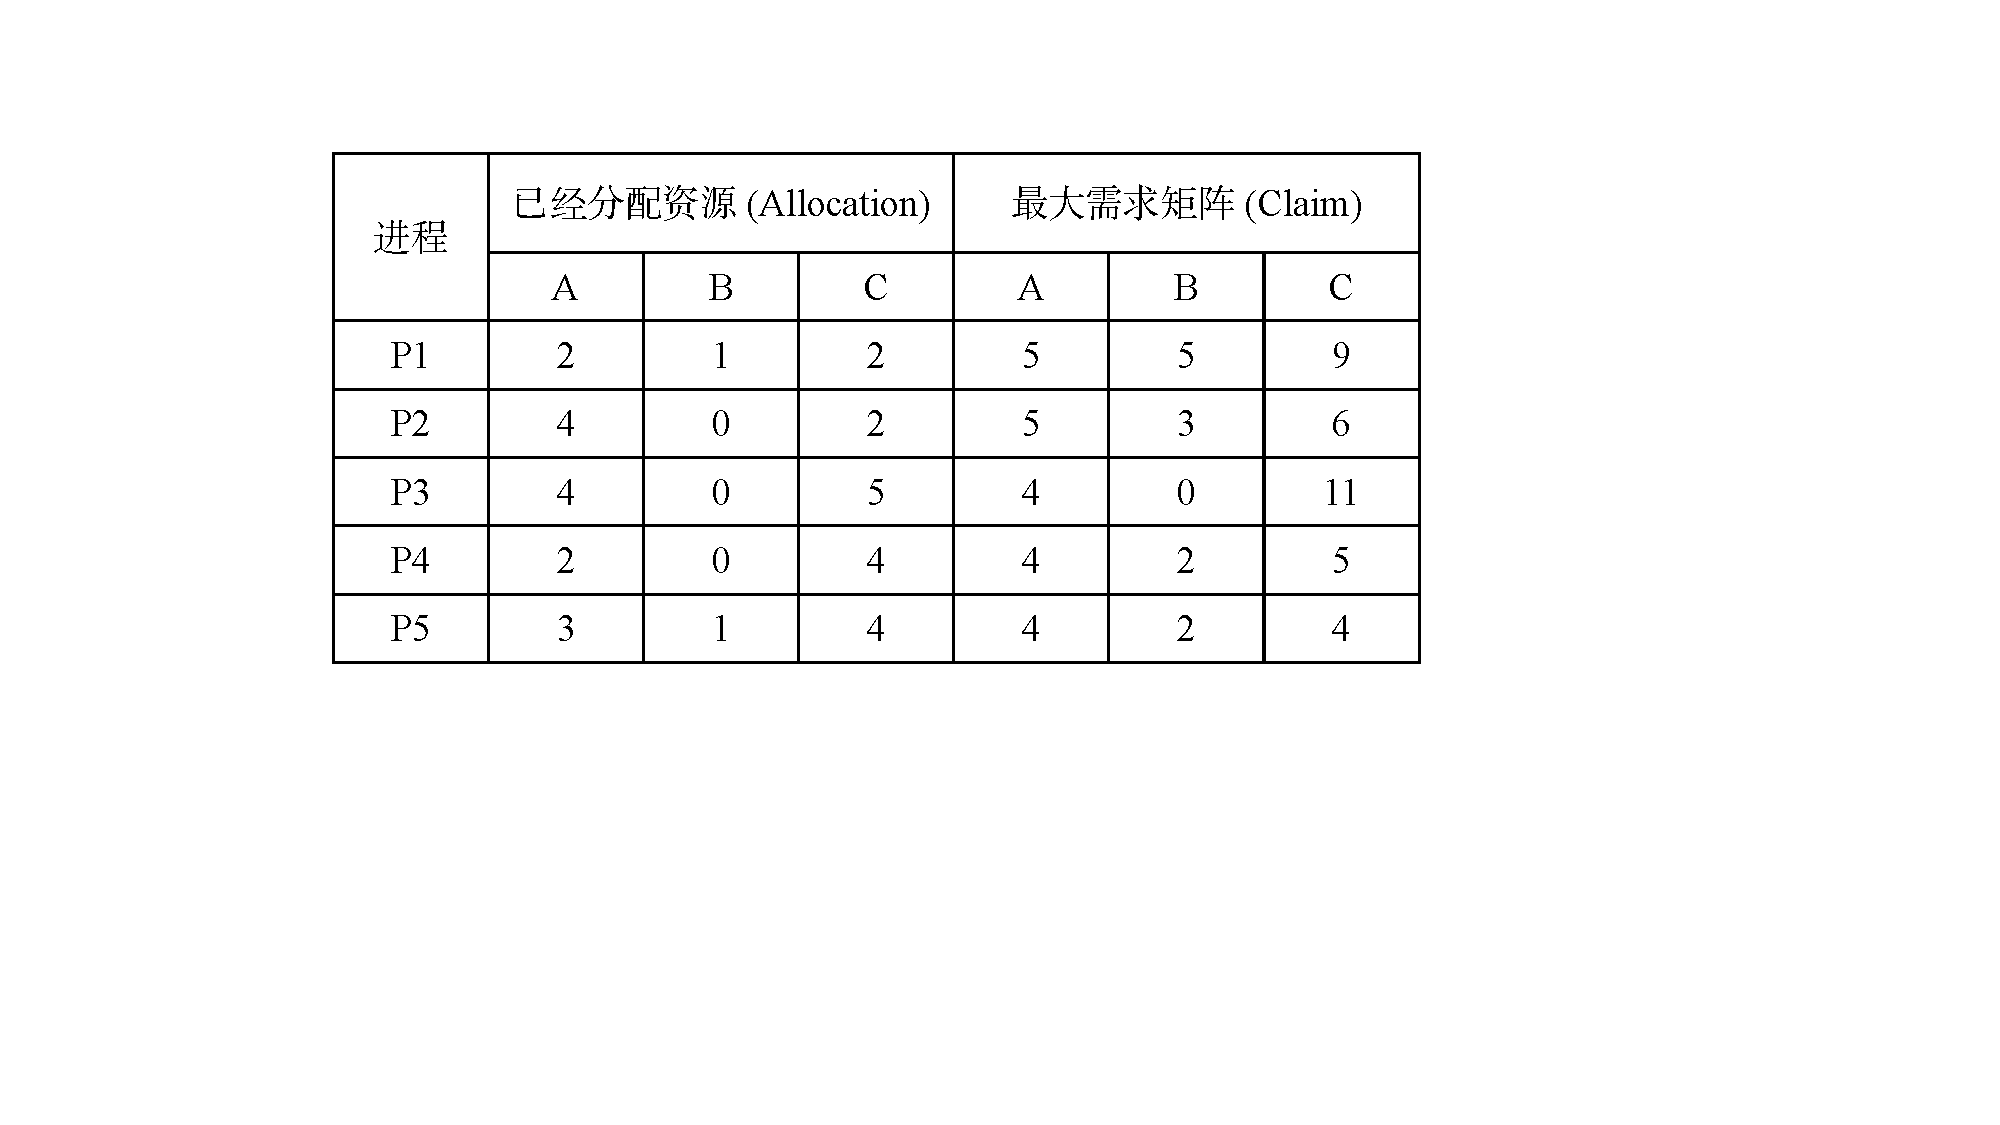
\includegraphics[width=0.5\linewidth]{期末考试第9题图.pdf}
        \vspace{-1em}
    \end{figure}
    \begin{enumerate}[label=(\arabic*)]
        \item $T_0$时刻的各资源剩余数量为多少?$T_0$时刻的是否为安全状态? 若是,请给出其中可能的一种安全序列,并依照该序列,写出各资源的回收步骤。
        \item 在$T_0$时刻,如果进程P1继续对A、B、C三类资源提出请求$Request(2, 2, 2)$后,系统能否将资源分配给P1进程?给出理由。
    \end{enumerate}

    
\end{problem}
    
\begin{solution}
    $T_0$时刻A资源的剩余量为$17-2-4-4-2-3=2$,B资源的剩余量为$5-1-1=3$,C资源的剩余量为$20-2-2-5-4-4=3$。

    $T_0$时刻为安全状态,其中的可能安全序列为P4$\rightarrow$P2$\rightarrow$P3$\rightarrow$P5$\rightarrow$P1

    \begin{figure}[H]
        \vspace{-0.5em}
        \centering
        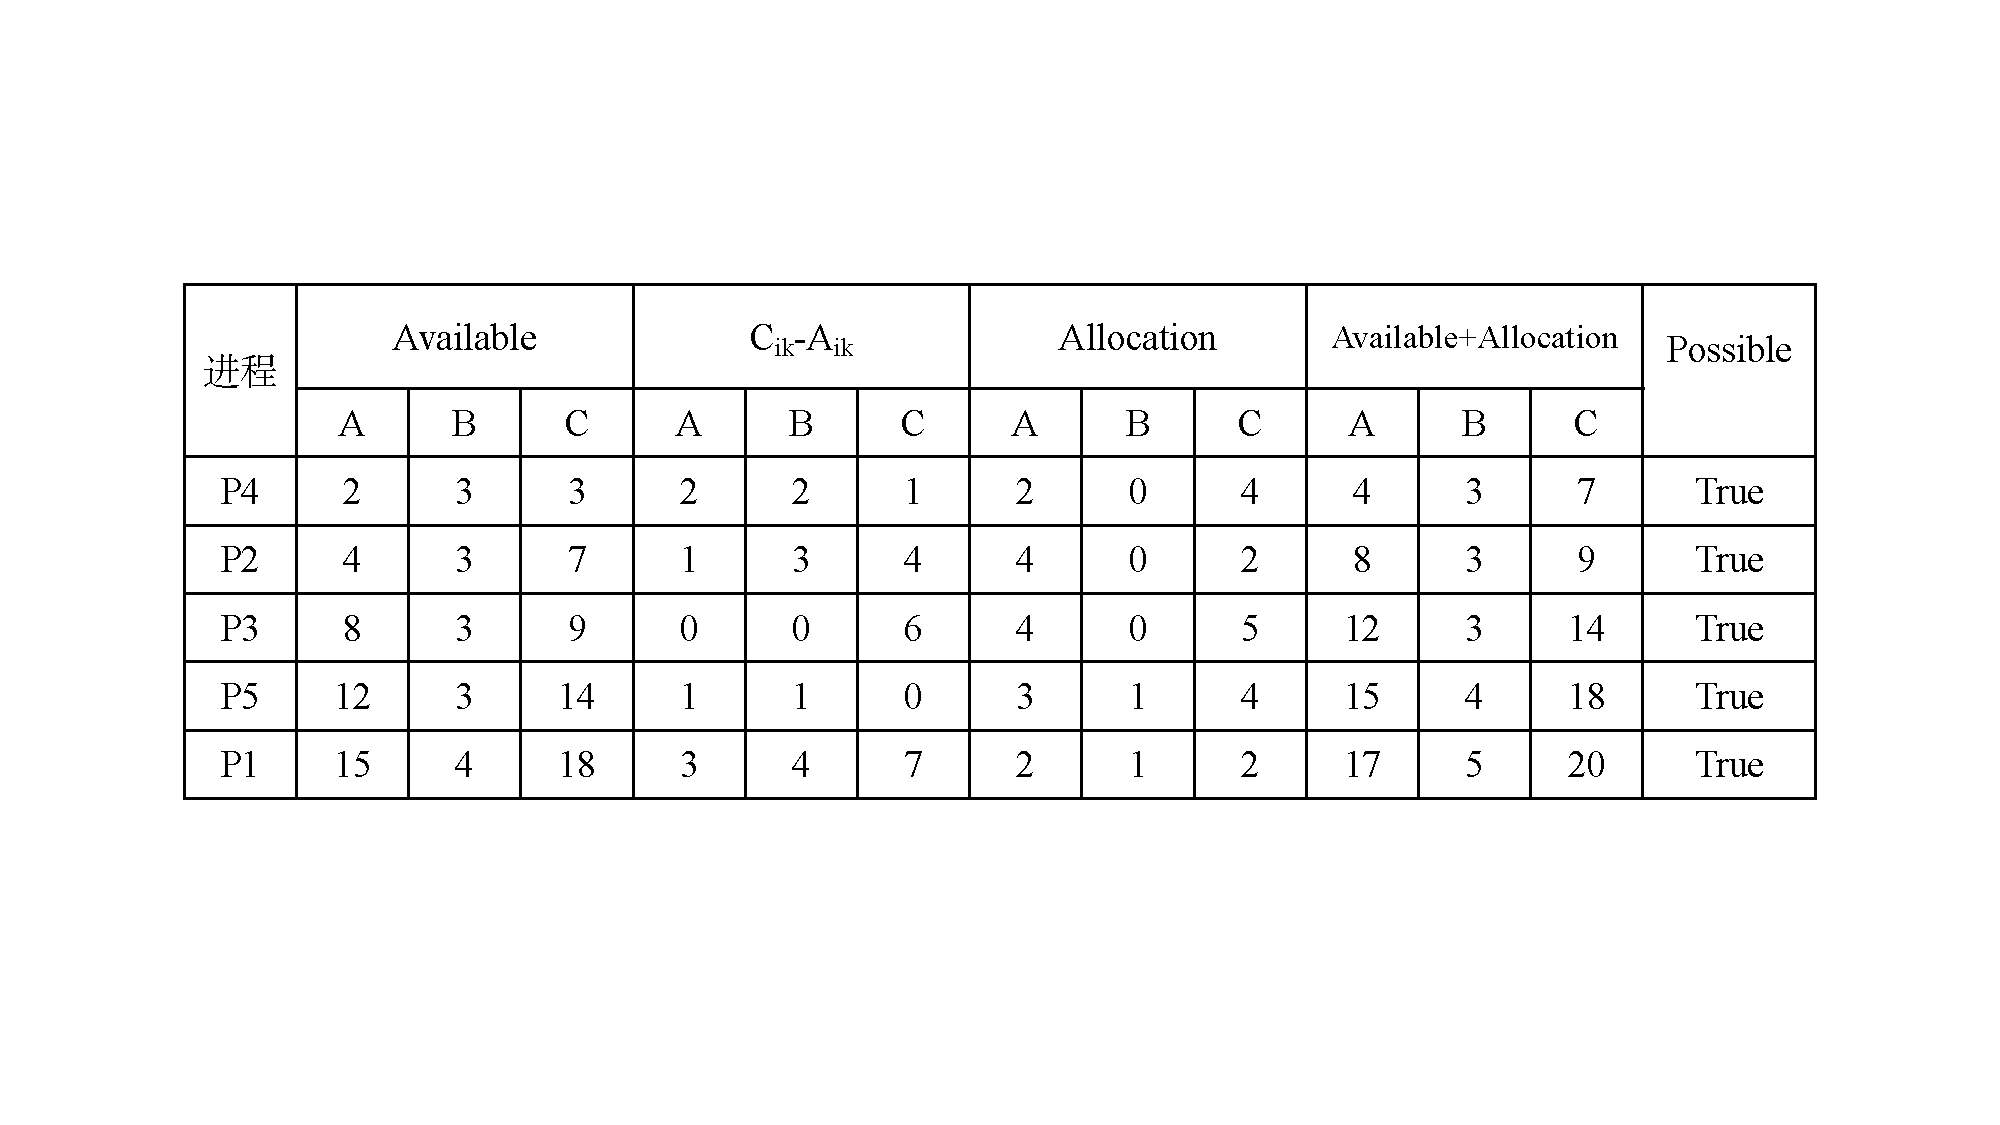
\includegraphics[width=0.8\linewidth]{期末考试第9题答案图.pdf}
        \vspace{-1em}
    \end{figure}

    在$T_0$时刻,假设满足P1的分配需求,此时$Available=(0,1,1)$,不能满足任何一个进程,系统处于不安全状态,因此不能分配。
\end{solution}




\end{document}